One way of visualizing some relations is by using a directed graph, which we define below.

\begin{definition}
A \textbf{directed graph} consists of two sets $V$ and $E \subset V \times V$. The set $V$ is called the set of vertices and the set $E$ is called the set of (directed) edges. 
\end{definition}

We can visualize a directed graph as follows. For visual purposes and a concrete example, we will consider the directed graph $V = \{a, b, c\}$ and $E = \{(a, a), (a, b), (b, c), (c, c)\}$. First, we imagine the objects of $V$ as dots.

\begin{figure}[ht]
	\centering
	
\includegraphics{Ch3/vertices.png}
\end{figure}

We can imagine each object $(x, y)$ of $E$ as a ``directed arrow'' (ie an arrow) where the back end of the arrow is $x$ and the front end of the arrow is $y$. For the example graph pictured this is visualized as follows.

\begin{figure}[ht]
	\centering
	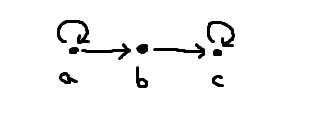
\includegraphics{Ch3/edges.png}
\end{figure}

In this way a graph can be visualized. One minor thing to observe is that any edge $(x, x)$ from an object $x$ to itself is drawn as a ``loop'' from the vertex starting at $x$ and pointing back at itself. The final thing to be observed is that any relation $R$ on a set $A$ can be seen as a graph. In this case, we take the vertices to be the set $A$ and we take the set of edges to be the set $R \subset A \times A$. We call this graph the \textbf{associated graph} of the relation $R$.

\begin{example}\label{gp1}
Suppose that a relation $R$ is transitive. Recall that a relation $R$ is transitive if for all $a, b, c \in A$, $(a, b) \in R, (b, c) \in R \implies (a, c) \in R$. What does this mean for its associated graph? Suppose then we have $a, b, c \in A$ with $(a, b) \in R, (b, c) \in R$. Then $(a, c) \in R$. A consequence of this is that if we have a chain of arrows from $a$ to $c$ then by transitivity there must be an arrow from $a$ to $c$ itself. This is illustrated in the picture below.
\end{example}
\begin{figure}[ht]
\centering
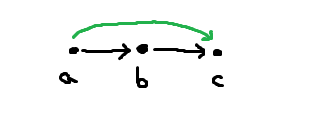
\includegraphics{Ch3/transitivity.png}
\end{figure}

%remark. For any a in R transitivity implies that any vertex that can be reached by ``travelling'' through $a$ can be reached through a in one step (this might require induction `formally').

\subsubsection{Exercises}

\begin{enumerate}
	\item Following the discussion of Example \ref{gp1}, interpret what it means for the associated graph of a relation $R$ if $R$ is 
	\begin{itemize}
		\item reflexive.
		\item symmetric.
	\end{itemize}
	\item Suppose Ryan presents you with the following graph associated with a relation $R$. He is very sad because the graph pictured is neither symmetric nor transitive. Add in the minimum number of necessary edges to make the relation\ldots
	\begin{itemize}
		\item reflexive.
		\item symmetric.
		\item transitive.
	\end{itemize}
\end{enumerate}
\begin{figure}[ht]
	\centering
	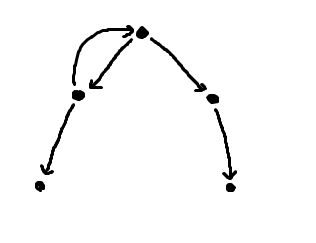
\includegraphics{Ch3/rgraph_ex1.png}
\end{figure}